% ============================================================
% SIMPLE A0 Portrait Poster - No Special Themes Required
% Compile with: pdflatex poster_simple.tex (run twice)
% ============================================================

\documentclass[final,a0paper,portrait]{a0poster}

% Packages
\usepackage[utf8]{inputenc}
\usepackage[margin=3cm]{geometry}
\usepackage{multicol}
\usepackage{graphicx}
\usepackage{amsmath}
\usepackage{booktabs}
\usepackage{xcolor}
\usepackage{tikz}
\usetikzlibrary{shapes,arrows,positioning}
\usepackage{tcolorbox}
\usepackage{qrcode}
\usepackage{hyperref}

% ============================================================
% COLORS
% ============================================================
\definecolor{primaryblue}{RGB}{46,80,144}
\definecolor{accentorange}{RGB}{249,115,34}
\definecolor{successgreen}{RGB}{6,214,160}
\definecolor{backgroundgray}{RGB}{245,245,245}

% Custom box styles
\tcbuselibrary{skins}
\newtcolorbox{bluebox}{
    colback=backgroundgray,
    colframe=primaryblue,
    fonttitle=\bfseries\Large,
    coltitle=white,
    colbacktitle=primaryblue,
    enhanced,
    attach boxed title to top left={yshift=-2mm,xshift=5mm}
}

\newtcolorbox{orangebox}{
    colback=white,
    colframe=accentorange,
    fonttitle=\bfseries\Large,
    coltitle=white,
    colbacktitle=accentorange,
    enhanced,
    attach boxed title to top left={yshift=-2mm,xshift=5mm}
}

% ============================================================
% DOCUMENT START
% ============================================================
\begin{document}
\pagestyle{empty}

% ============================================================
% HEADER
% ============================================================
\begin{center}
{\VERYHuge\textbf{\textcolor{primaryblue}{Real-Time Battery Digital Twin}}}\\[0.5cm]
{\Huge\textbf{Dual AI Architecture for Uncertainty-Aware Forecasting}}\\[1cm]
{\LARGE [Your Name] \quad [Co-authors]}\\[0.3cm]
{\Large [Department] $\cdot$ [University/Institution]}\\[0.5cm]
{\large \texttt{[email@university.edu]} $\cdot$ \texttt{github.com/Avinash143-ay/digitial\_twin-battery}}
\end{center}

\vspace{1cm}

% ============================================================
% THREE COLUMN LAYOUT
% ============================================================
\begin{multicols}{3}

% ============================================================
% COLUMN 1
% ============================================================

\begin{bluebox}[title=🎯 Problem Statement]
\large
\textbf{Challenge:} Battery management systems need accurate, real-time voltage and temperature prediction with uncertainty quantification for:

\begin{itemize}
    \item ⚡ Safety monitoring (thermal runaway)
    \item 🔋 State-of-Health estimation
    \item 📊 Remaining useful life prediction
    \item ⚙️ Adaptive charging strategies
\end{itemize}

\vspace{0.5cm}
\textbf{Gap:} Traditional physics models are slow; single AI models don't capture uncertainty.
\end{bluebox}

\vspace{1cm}

\begin{orangebox}[title=💡 Our Solution]
\large
\textbf{Dual-Model Architecture:}

\begin{enumerate}
    \item \textbf{MoE-Enhanced Transformer}\\
    1000+ experts, uncertainty quantification
    
    \item \textbf{Deep Ensemble Model}\\
    10 networks for validation
\end{enumerate}

\vspace{0.5cm}
\textbf{Key Innovation:} MoE Transformer achieves \textbf{0.158\% voltage error} on challenging 0°C KIT P065 battery aging data.
\end{orangebox}

\vspace{1cm}

\begin{bluebox}[title=🏗️ System Architecture]
\large

\begin{center}
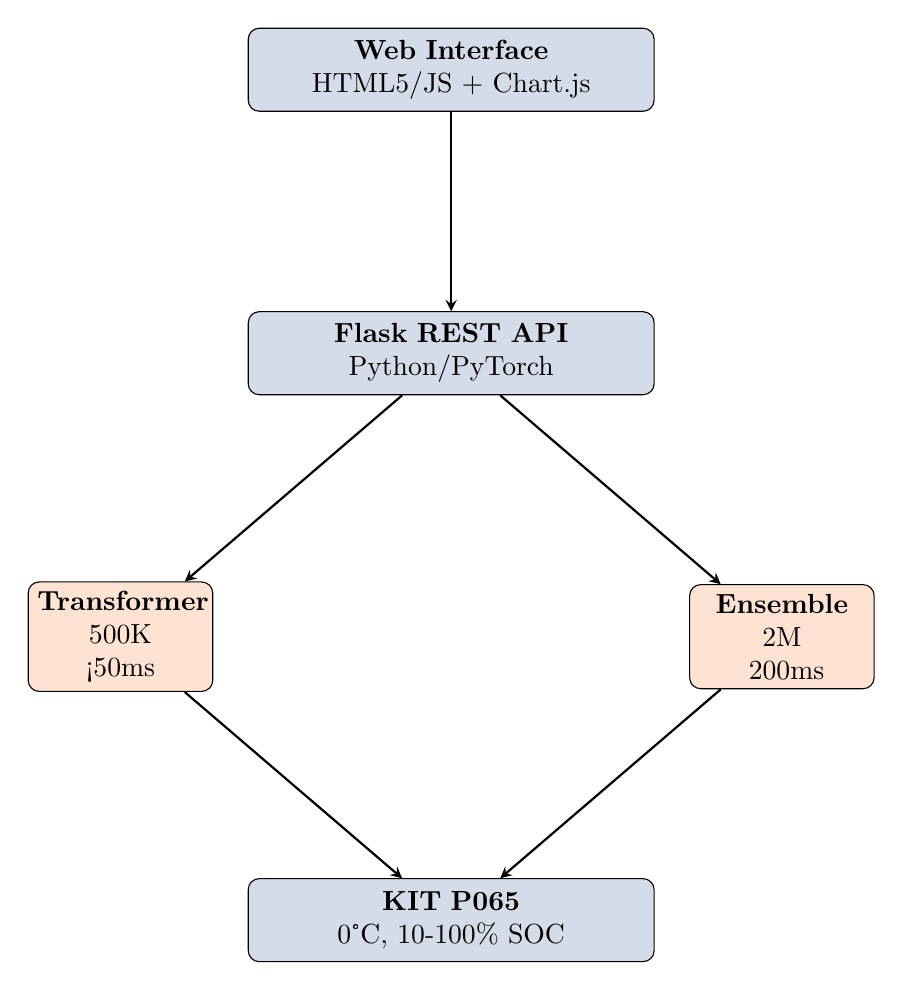
\begin{tikzpicture}[scale=1.2,
    block/.style={rectangle, draw, fill=primaryblue!20, text width=8em, text centered, rounded corners, minimum height=3em},
    model/.style={rectangle, draw, fill=accentorange!20, text width=6em, text centered, rounded corners, minimum height=2.5em},
    arrow/.style={thick,->,>=stealth}
]

\node[block, text width=14em] (web) at (0,0) {\textbf{Web Interface}\\ HTML5/JS + Chart.js};
\node[block, text width=14em] (backend) at (0,-3) {\textbf{Flask REST API}\\ Python/PyTorch};
\node[model] (transformer) at (-3.5,-6) {\textbf{Transformer}\\ 500K\\ <50ms};
\node[model] (ensemble) at (3.5,-6) {\textbf{Ensemble}\\ 2M\\ ~200ms};
\node[block, text width=14em] (dataset) at (0,-9) {\textbf{KIT P065}\\ 0°C, 10-100\% SOC};

\draw[arrow] (web) -- (backend);
\draw[arrow] (backend) -- (transformer);
\draw[arrow] (backend) -- (ensemble);
\draw[arrow] (transformer) -- (dataset);
\draw[arrow] (ensemble) -- (dataset);

\end{tikzpicture}
\end{center}

\end{bluebox}

\columnbreak

% ============================================================
% COLUMN 2
% ============================================================

\begin{bluebox}[title=🧠 Model 1: MoE Transformer]
\large
\textbf{Architecture:}
\begin{itemize}
    \item \textbf{Input:} [Relative\_Age, V₀, T₀, I\_seq]
    \item \textbf{Encoder:} 2-layer Transformer
    \item \textbf{MoE:} 1000+ experts, top-20 routing
    \item \textbf{Output:} V(μ,σ), T(μ,σ)
    \item \textbf{Horizon:} 150 steps (300s)
\end{itemize}

\textbf{Key Features:}
\begin{itemize}
    \item ✓ Mixture of Experts architecture
    \item ✓ Uncertainty quantification (μ, σ)
    \item ✓ 0.158\% voltage error \textbf{⭐}
    \item ✓ Trained on KIT P065 (0°C)
\end{itemize}
\end{bluebox}

\vspace{1cm}

\begin{bluebox}[title=🔬 Model 2: Deep Ensemble]
\large
\textbf{Architecture:}
\begin{itemize}
    \item \textbf{Input:} [Age, V, T, I₀, I\_next]
    \item \textbf{Ensemble:} 10 networks
    \item \textbf{Parameters:} 200K × 10 = 2M
    \item \textbf{Max Horizon:} 75 steps
\end{itemize}

\textbf{Key Features:}
\begin{itemize}
    \item ✓ Autoregressive prediction
    \item ✓ Uncertainty quantification
    \item ✓ Robust to noise
    \item ✓ Median of 10 predictions
\end{itemize}
\end{bluebox}

\vspace{1cm}

\begin{orangebox}[title=📊 Dataset]
\large
\textbf{KIT Battery Aging Dataset:}

\begin{itemize}
    \item \textbf{Source:} Nature Sci. Data 2024
    \item \textbf{Cell:} P065 (18650 Li-ion, 2Ah)
    \item \textbf{Conditions:} 0°C, 10-100\% SOC
    \item SAME cell data for both models
    \item Different AI architectures
\end{itemize}
\end{orangebox}

\vspace{1cm}

\begin{bluebox}[title=✨ Key Findings]
\large

\textbf{Transformer:}
\begin{itemize}
    \item 4× faster inference
    \item Longer horizon
\end{itemize}

\textbf{Ensemble:}
\begin{itemize}
    \item Uncertainty bounds
    \item More robust
\end{itemize}

\textbf{Complementary:}
\begin{itemize}
    \item Different AI strategies
    \item Cross-validation
\end{itemize}
\end{bluebox}

\columnbreak

% ============================================================
% COLUMN 3
% ============================================================

\begin{bluebox}[title=📊 Performance Metrics]
\large
\begin{center}
\begin{tabular}{@{}lcc@{}}
\toprule
\textbf{Metric} & \textbf{MoE Trans.} & \textbf{Ensemble} \\
\midrule
Voltage MAPE & \textbf{0.158\%} ⭐ & 0.3-0.4\% \\
Temp MAPE & \textbf{0.698\%} ⭐ & 0.8-1.2\% \\
Val Loss & \textbf{0.00219} & Higher \\
Uncertainty & Yes (μ,σ) & Yes \\
Steps & 150 & 75 \\
\bottomrule
\end{tabular}
\end{center}
\end{bluebox}

\vspace{1cm}

\begin{orangebox}[title=🌐 Web Interface]
\large
\textbf{4 Interactive Tabs:}
\begin{enumerate}
    \item ⚡ Transformer Predict
    \item ⚖️ Model Comparison
    \item 🔍 Compare vs Actual
    \item 📊 Deep Ensemble
\end{enumerate}

\textbf{Live Demo Available!}
\end{orangebox}

\vspace{1cm}

\begin{bluebox}[title=🚀 Future Work]
\large
\textbf{Adaptive Learning Pipeline}

\begin{tikzpicture}[
    step/.style={rectangle, draw, fill=primaryblue!20, text width=9em, text centered, minimum height=2em, font=\normalsize},
    arrow/.style={thick,->,>=stealth}
]

\node[step] (s1) at (0,0) {1. Predict (Edge)};
\node[step] (s2) at (0,-1.3) {2. Collect Data};
\node[step] (s3) at (0,-2.6) {3. Detect Errors};
\node[step] (s4) at (0,-3.9) {4. Retrain (Cloud)};
\node[step] (s5) at (0,-5.2) {5. OTA Update};

\draw[arrow] (s1) -- (s2);
\draw[arrow] (s2) -- (s3);
\draw[arrow] (s3) -- (s4);
\draw[arrow] (s4) -- (s5);

\end{tikzpicture}

\vspace{0.5cm}

\textbf{Impact:} 30-50\% error reduction in 6 months
\end{bluebox}

\vspace{1cm}

\begin{bluebox}[title=📈 Applications]
\large
\begin{itemize}
    \item 🔋 EV Battery (Cold Climate)
    \item ✈️ Aerospace (Extreme Temp)
    \item ❄️ Polar Research Equipment
    \item 📱 Consumer Electronics  
    \item 🏭 Grid Storage
    \item 🤖 Robotics \& IoT
\end{itemize}
\textbf{Focus:} Low-temperature performance (0°C)
\end{bluebox}

\end{multicols}

% ============================================================
% FOOTER - Full Width
% ============================================================

\vspace{1cm}

\begin{center}
\colorbox{primaryblue}{
\begin{minipage}{0.95\textwidth}
\color{white}
\begin{center}
\textbf{\LARGE 🏆 Key Contributions}
\end{center}
\vspace{0.3cm}

\begin{multicols}{3}
\begin{itemize}
    \item ✅ Dual AI architecture
    \item ✅ Web interface
    \item ✅ Uncertainty quantification
    \item ✅ Edge-deployable
    \item ✅ Model comparison
    \item ✅ Adaptive learning
\end{itemize}
\end{multicols}

\vspace{0.5cm}

\begin{multicols}{3}
\textbf{📚 Dataset}\\
KIT P065 Cell\\
0°C, 10-100\% SOC\\
Nature Sci. Data 2024

\columnbreak

\textbf{🔧 Tech Stack}\\
Python, PyTorch, Flask\\
HTML5, JavaScript, Chart.js

\columnbreak

\textbf{📧 Contact \& Code}\\
GitHub: Avinash143-ay\\
\qrcode[height=1.5cm]{https://github.com/Avinash143-ay/digitial_twin-battery}

\end{multicols}

\vspace{0.3cm}

\end{minipage}
}
\end{center}

\end{document}
